
\chapter{Introduction}

In this intermediate report we describe the activities to formally verify
the correctness of parts of the software developed in the OpenETCS project.

While major parts of the functionality of {Subset 026} are modelled in 
higher-level languages, there is also a substantial part of \emph{supporting} software
that is developed in the~C programming language.

In this document we report about results on the verification of that C~code.
In particular, we report on the use of static analysis methods (including formal methods)
on C~code that has been developed by the project partner Siemens.

\begin{figure}[hbt]
\begin{center}
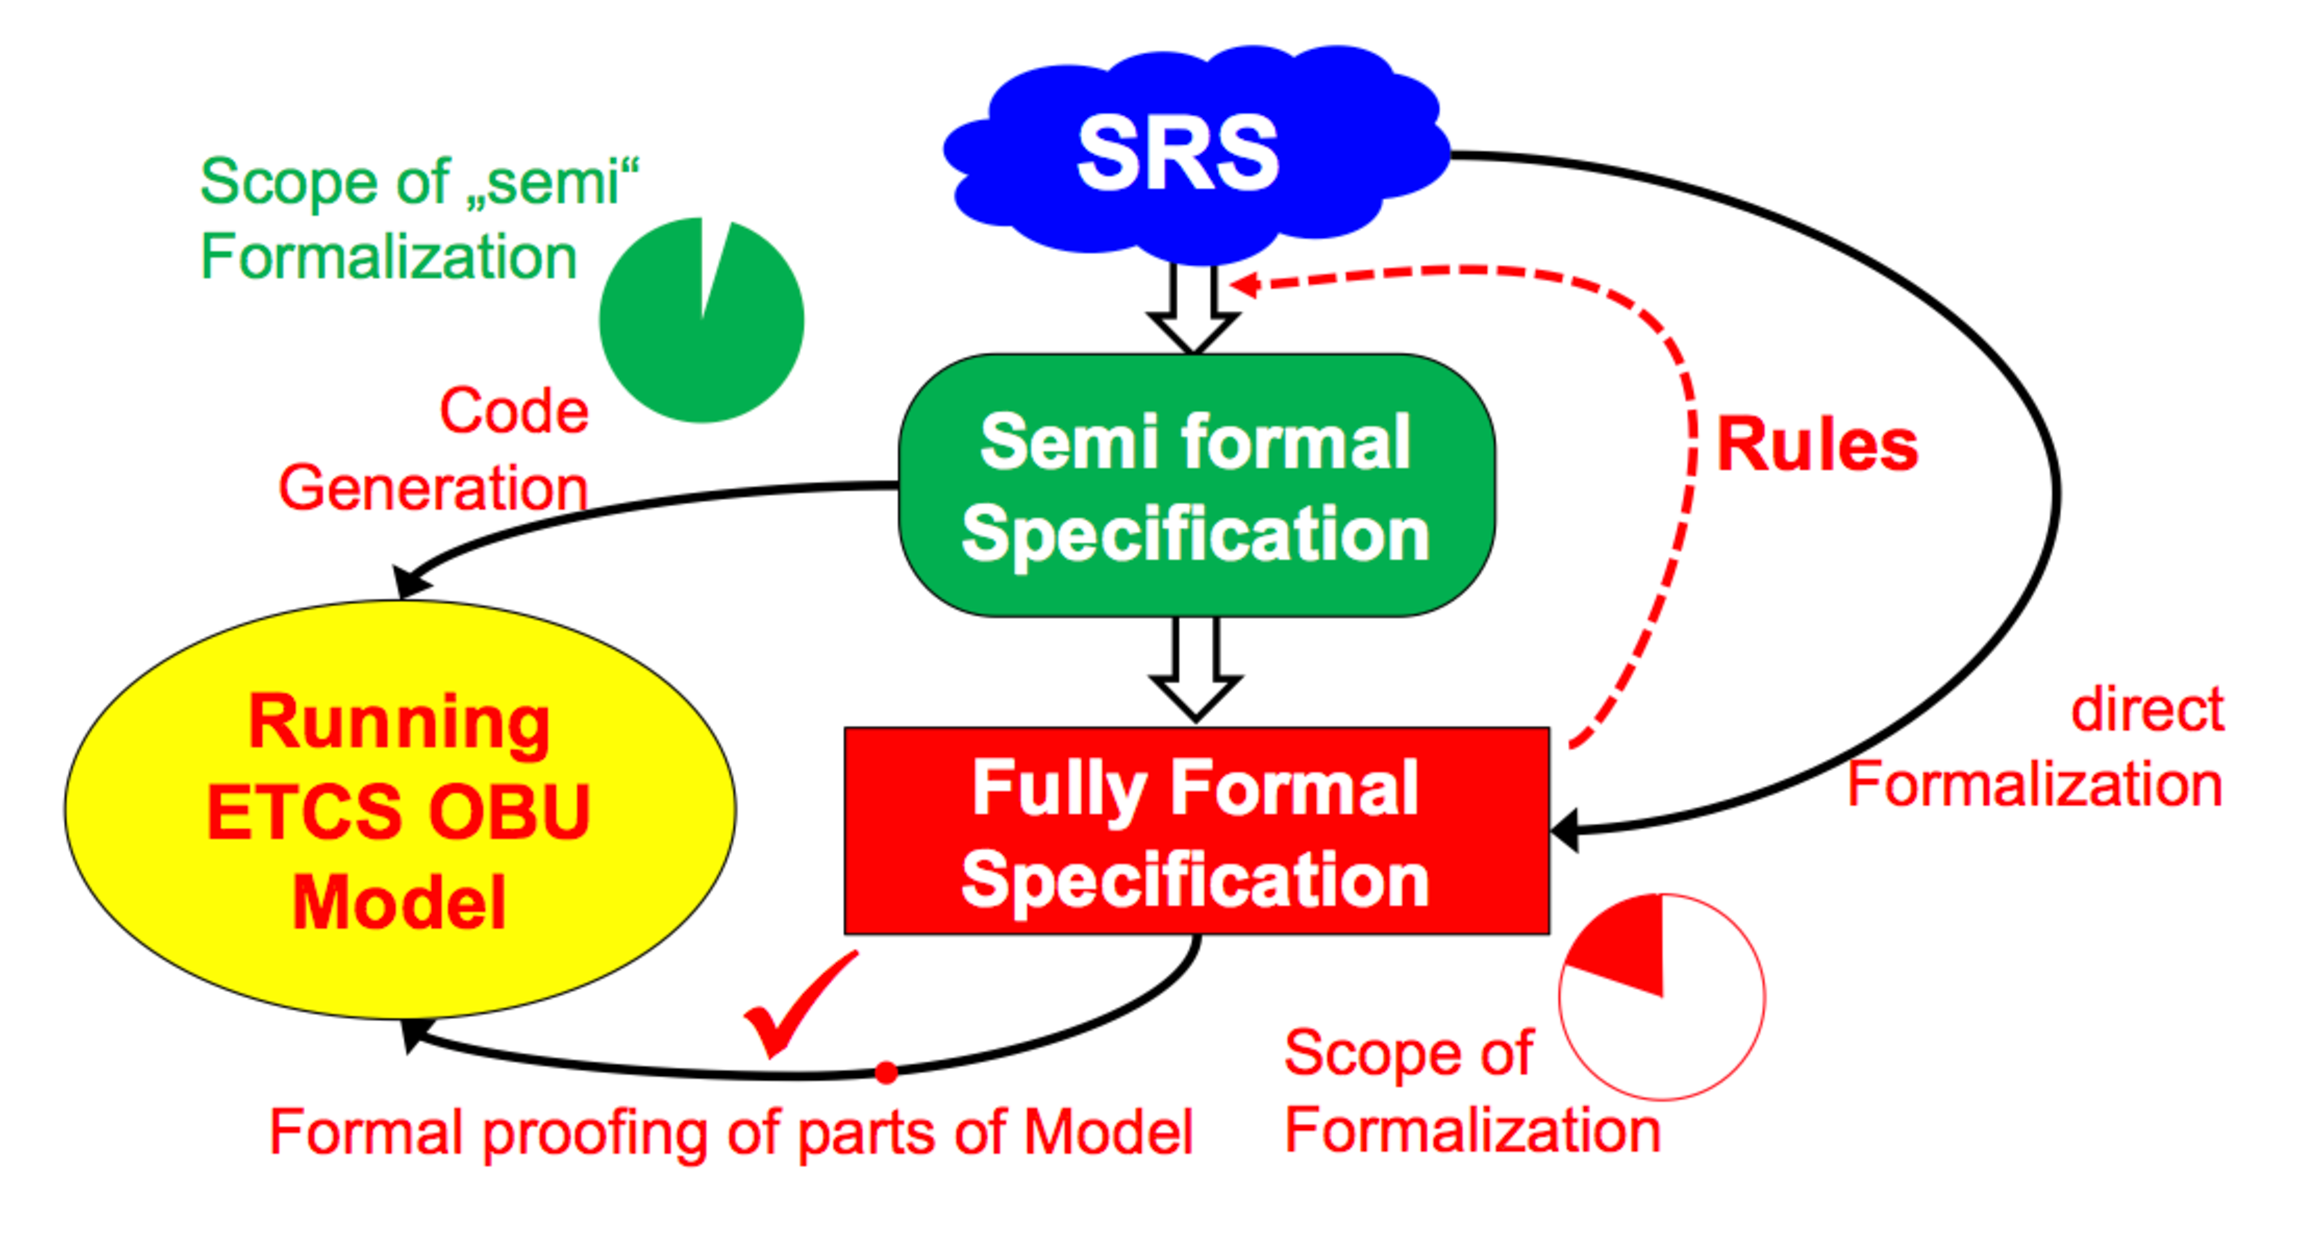
\includegraphics[width=0.95\textwidth]{figures/scope-of-formalization.pdf}
\caption{\label{fig:scope-of-formalization} Scope of formal methods with in OpenETCS}
\end{center}
\end{figure}

Figure~\ref{fig:scope-of-formalization} outlines the roles of formal methods
within the OpenETCS project.
What this figure shall convey is that even a subsystem such as described by
\emph{Subset 026} of the ETCS specification
is usually too complex to be completely formally specified.
Therefore, \emph{semi-formal modelling techniques} and \emph{tests} and 
\emph{simulations} play a crucial role to verify that the implementation
satisfies its specification.
However, for clearly defined modules and select system properties, formal methods
can well be applied to establish the correctness of an implementation.

Figure~\ref{fig:scope-of-code-verification} shows slightly more detailed
the OpenETCS software.
The report at hand is limited to the parts encapsulated by C software encapsulated 
in a \fbox{dashed box}.

\clearpage

\begin{figure}[hbt]
\begin{center}
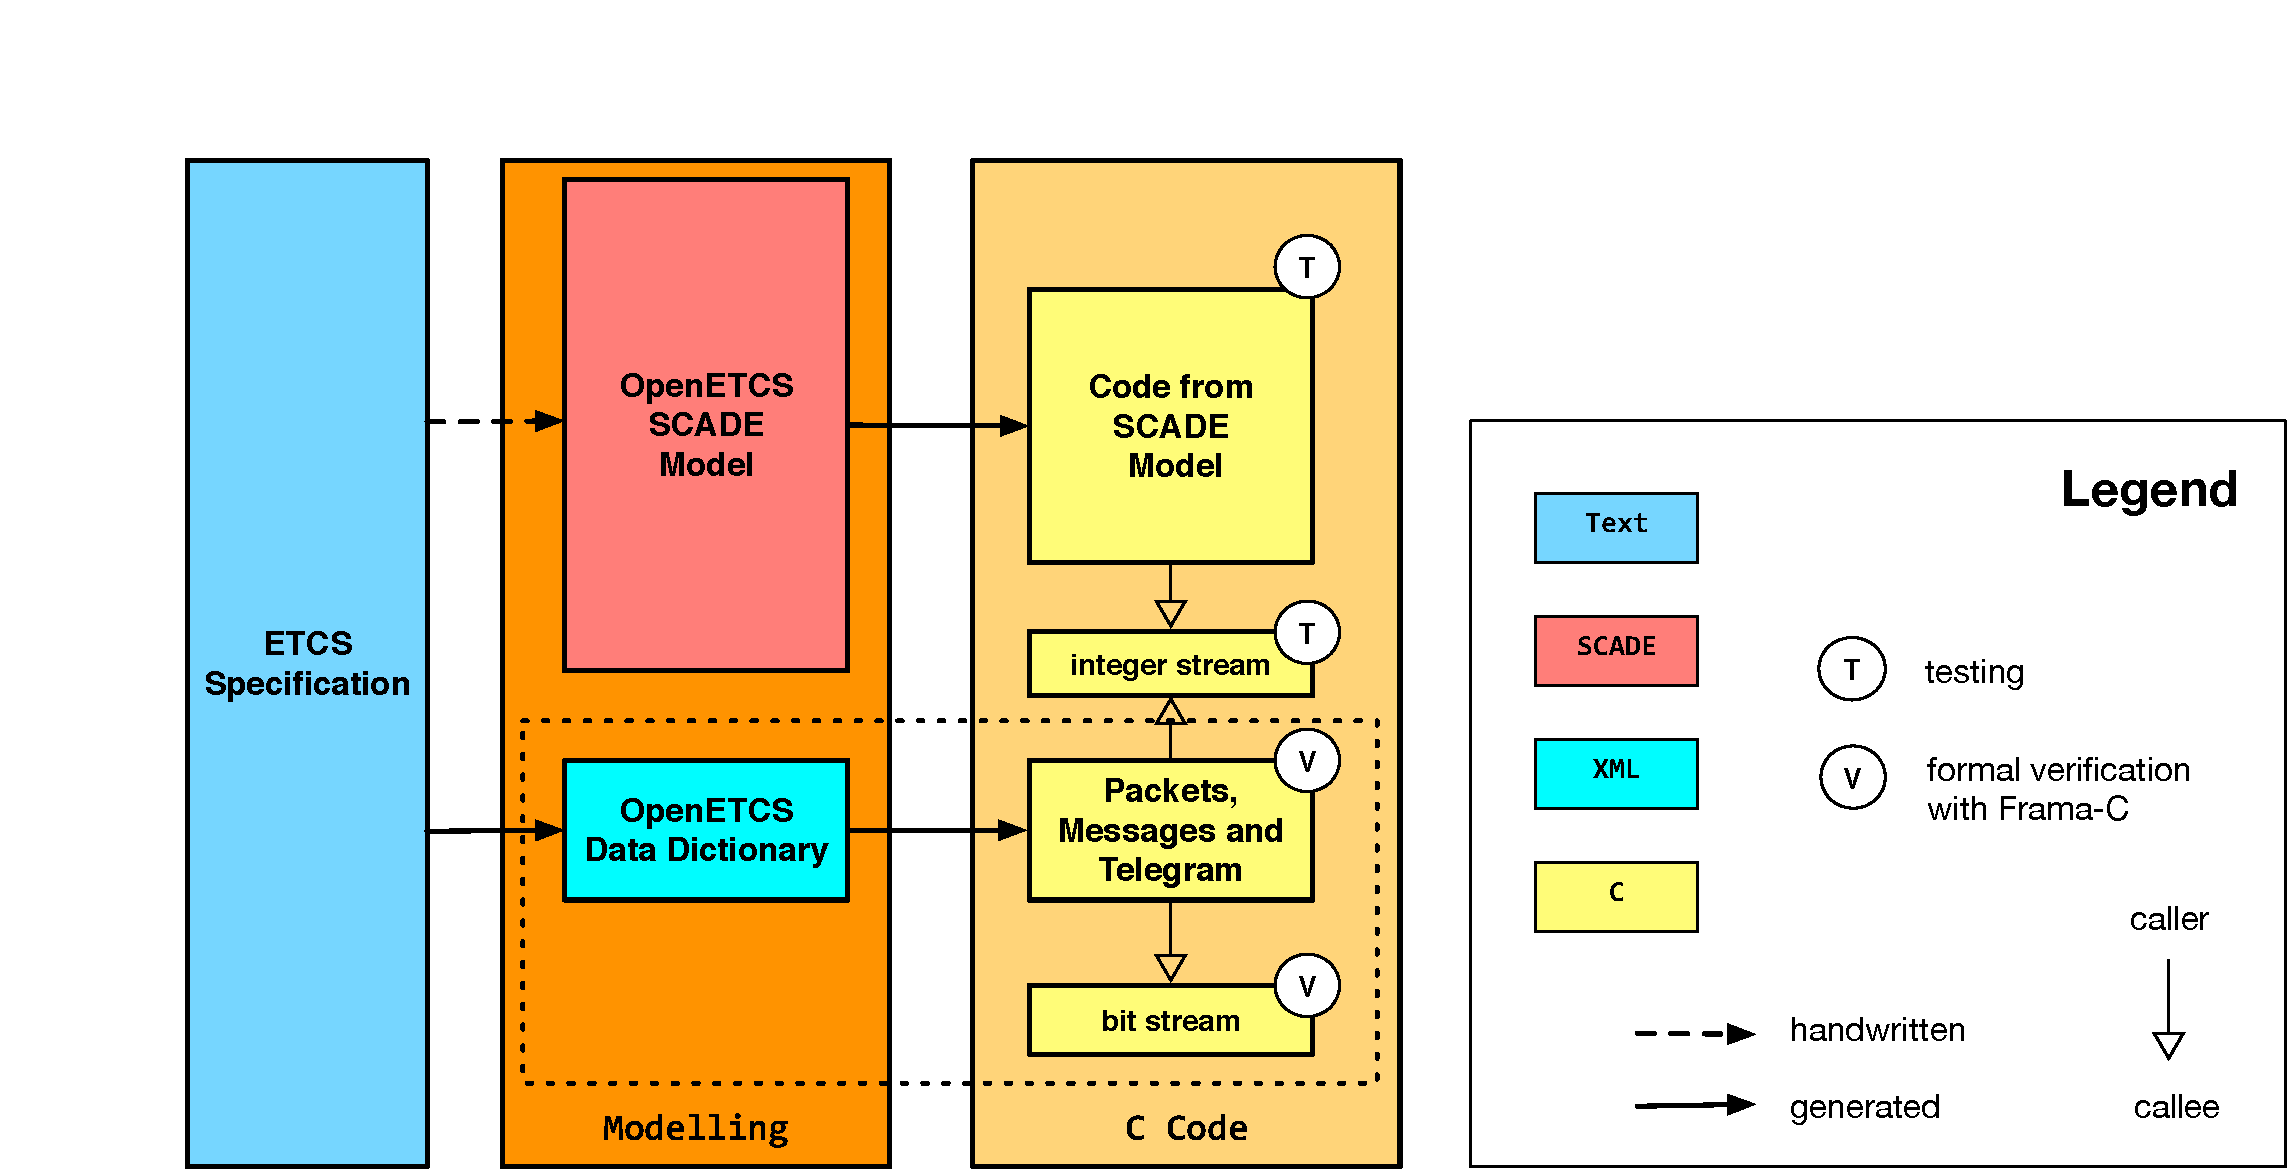
\includegraphics[width=0.95\textheight,angle=90]{figures/OpenETCS-Stack.pdf}
\caption{\label{fig:scope-of-code-verification} Scope of code verification}
\end{center}
\end{figure}

\FloatBarrier

\section{Software layers}

Figure~\ref{fig:software-layers} shows the layer structure of the OpenETCS C~code.
The OpenETCS decoder\slash enocder is a collection of data structures and associated functions
for reading and writing ETCS packets from\slash to a bit stream.

\begin{figure}[hbt]
\begin{center}
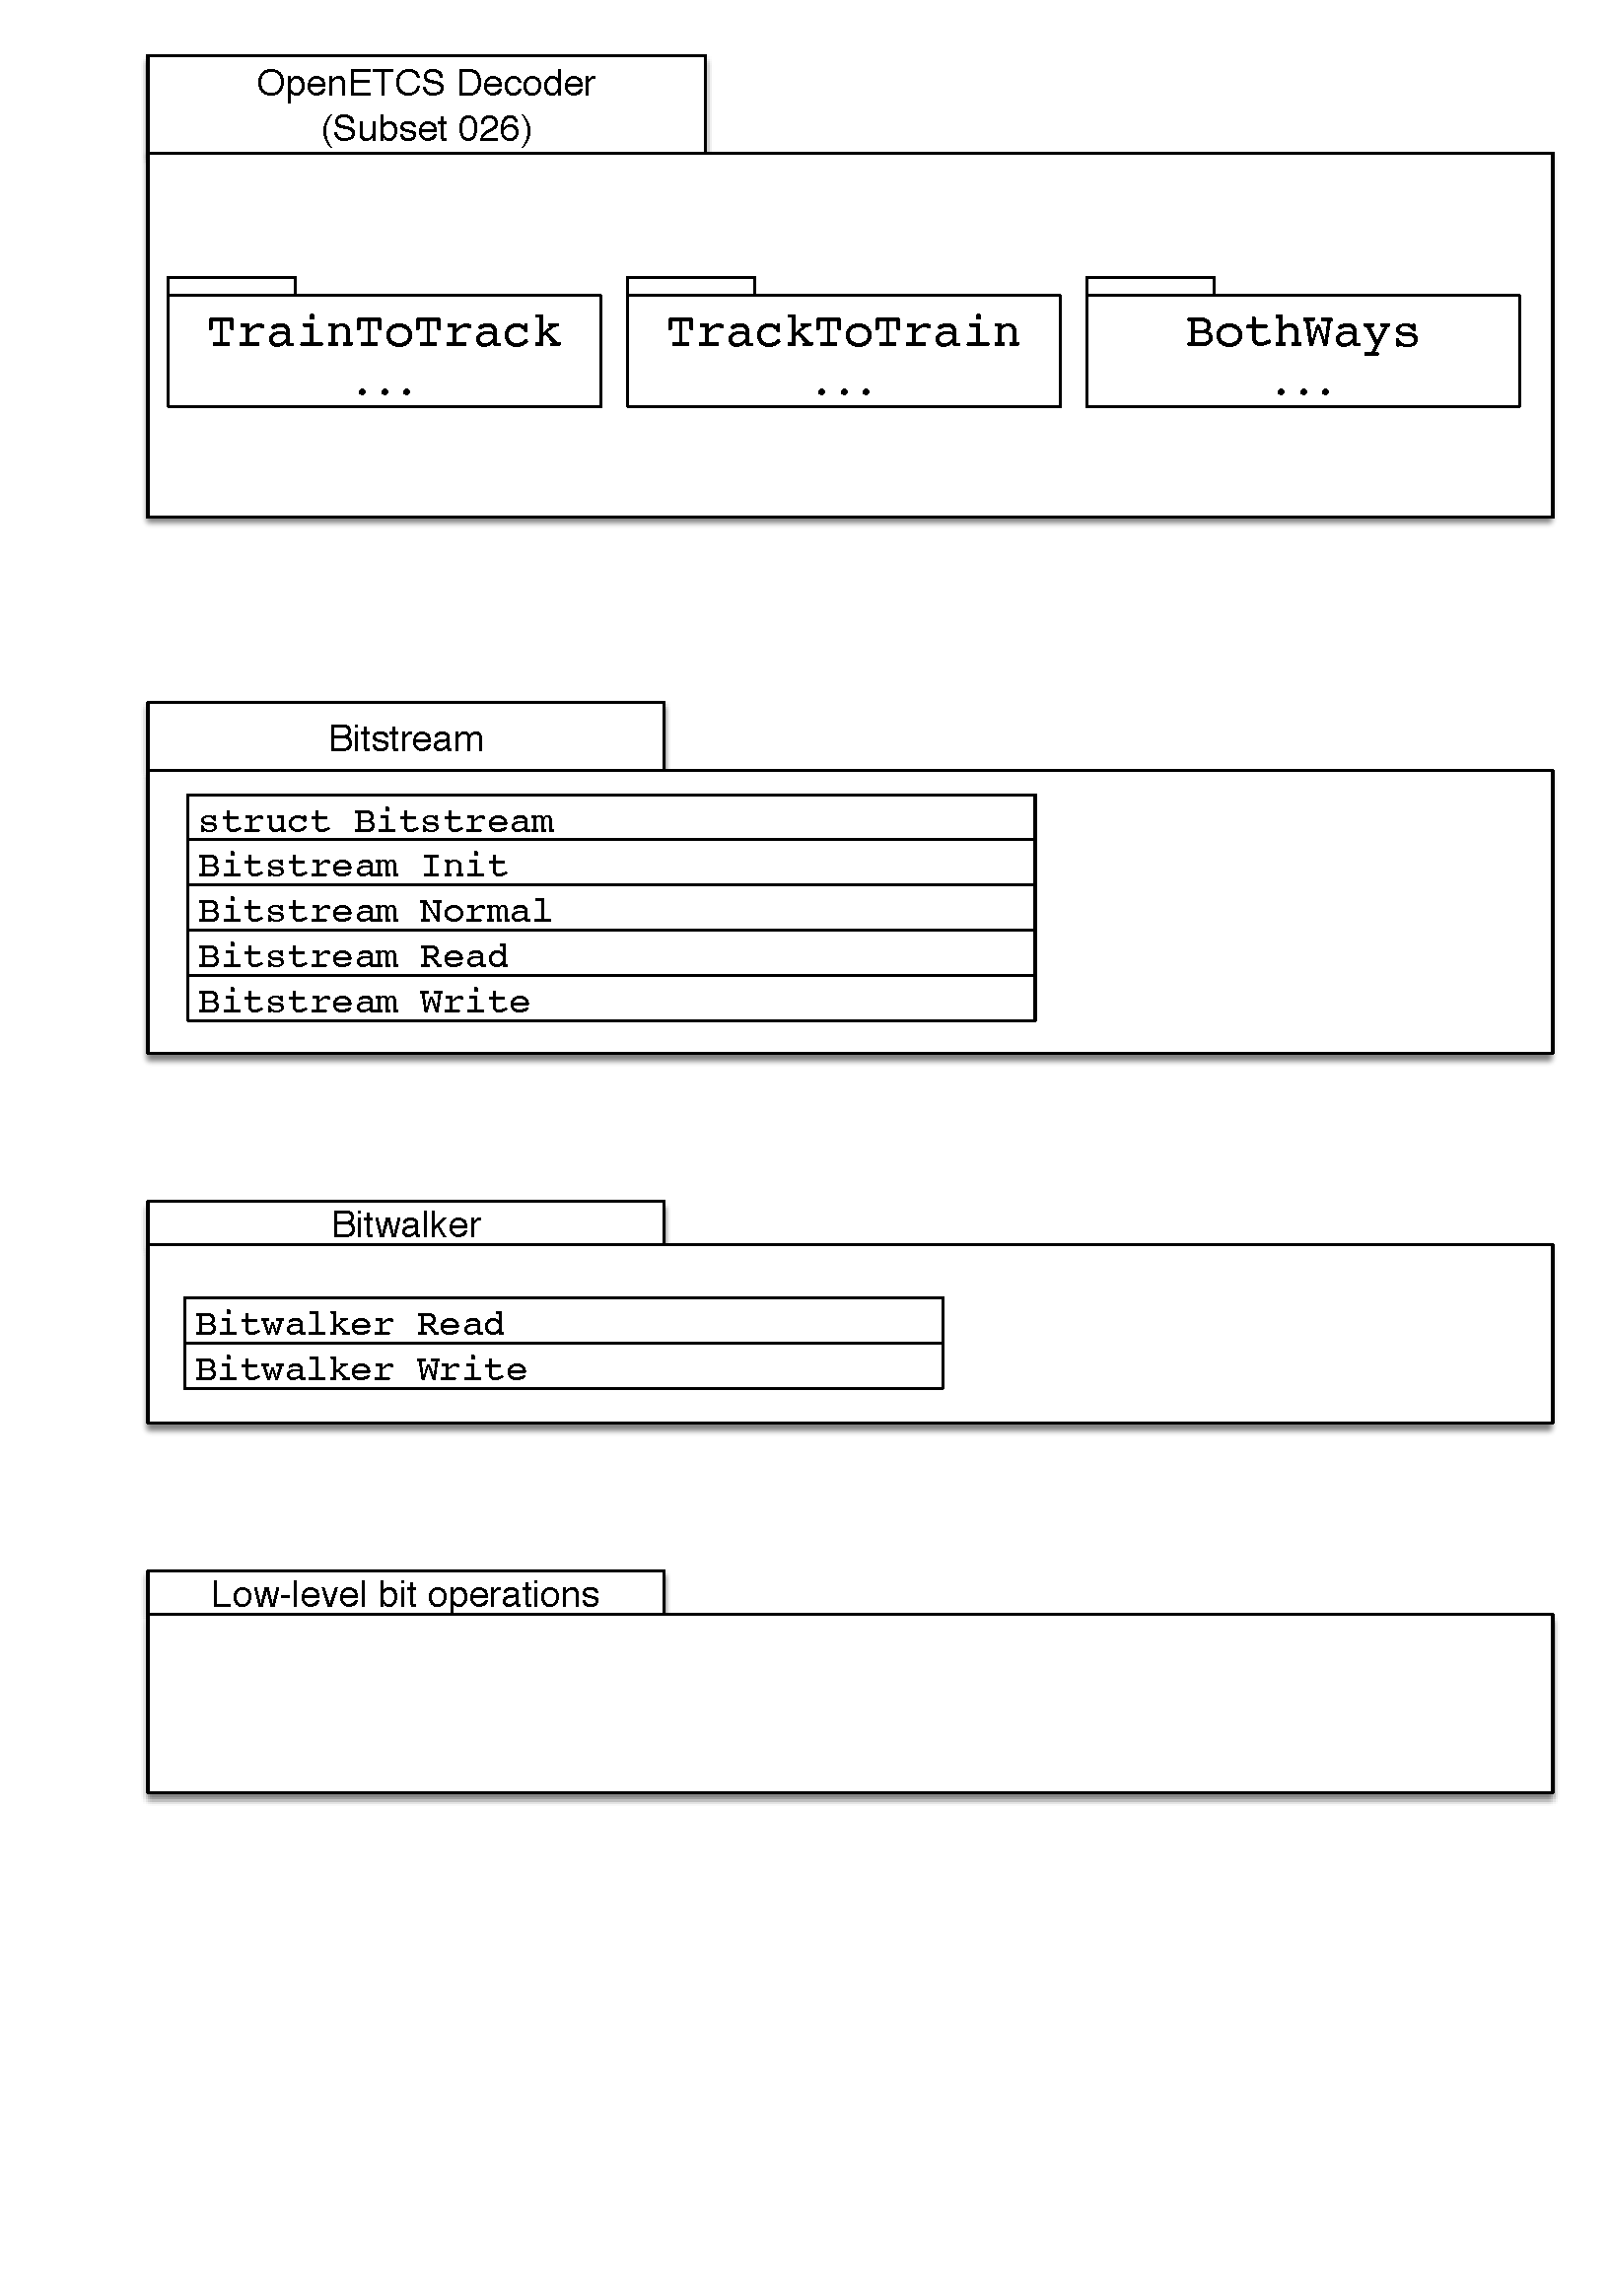
\includegraphics[width=1.0\textwidth]{figures/software-layers.pdf}
\caption{\label{fig:software-layers} Software layers of the OpenETCS C~code}
\end{center}
\end{figure}

\FloatBarrier

In order to fulfill their task the decoder and encoder function rely on an
implementation of bit streams in C.
The \inl{Bitstream} package in turn is built on top of the so-called \emph{bitwalker} layer.
In order to accomplish the task of formal verification of these layers 
we also provided several functions that read and write individual bits for basic C~types.

This software has been analyzed by the OpenETCS project partners SQS (Spain)
and Fraunhofer FOKUS (Germany).
SQS used several static analysis tools to identify defects and to derive useful metrics.
Fraunhofer FOKUS, on the other hand, used the \framac tool set,
which is developed by the French project partner \cealist,
in order to \emph{formally verify} various properties of the \bitwalker.

These analyses contribute to the ultimate verification goals, which are the following:

\begin{enumerate}
\item provide evidence that the Bitwalker software satisfies 
      accepted quality standards
\item develop a formal specification for the Bitwalker software
\item verify that the Bitwalker software satisfies its formal specification
\item show that the Bitwalker software does not raise runtime errors
\item verify that OpenETCS decoder calls the Bitwalker software only
      according to its specification
\end{enumerate}

We are confident that all these verification goals can be reached.
For this preliminary verification report,
we provide partial answers to the first four topics.
In order to achieve the last goal, more development and verification
work is currently conducted by Fraunhofer ESK and Fraunhofer FOKUS. 

\section{Structure of this document}

Chapter~\ref{sec:frama-c} gives a short overview on the \framacwp tool
that plays a central role in the verification of the Bitwalker functions.
Here we also try to rectify some misunderstandings about formal verification
that we have encountered in our work.

In Chapter~\ref{sec:formal-verification} we analyze
the functions \peek and \poke from the Bitwalker core and
\begin{enumerate}
\item formally specify the
      expected functional behavior in the \acsl specification language of {Frama-C}
      and
\item report on the formal proof 
	that these
      C~functions do not raise runtime errors when called according to their
      formal specification, established using 
      the {Frama-C} verification platform.
\end{enumerate}

So far only a part of Siemens' \bitwalker has been formalized and verified.
In the process of this work several enhancements for the \framac verification platform
have been identified and reported to the developers at {CEA LIST}.

In Chapter~\ref{sec:static-analysis}, we report about the results of
SQS' application of a broad range of static analysis tools on the \bitwalker. 
In contrast to \framac, these tools cannot exhaustively
detect all potential defects of a given kind.
Nevertheless, these they are very useful at finding well-known quality deficiencies that
might occur in C or \CC\ software.

In Chapter~\ref{sec:conclusions}, we draw conclusions from this preliminary work
and outline the next steps in our verification efforts.

